%!TEX root = main.tex

\section{Overview}
\labsection{overview}

\er{write a short intro to section}

%%%%%%%%%%%%%%%%%%%%%%%%%%%%%%%%%%%%%%%%%%%%%%%%%%%%%%%%%%

\begin{algorithm}
	\footnotesize
	\DontPrintSemicolon
	
	$\AlgoSend   ($\Ms: \Msg) : \VoidType  \tcp*[1]{send to all nodes in wireless range}
	$\FuncHandler($\Ms: \Msg) : \VoidType  \tcp*[1]{callback when a message is received}

\caption{\labalg{network_api}Network layer API}
\end{algorithm}

%%%%%%%%%%%%%%%%%%%%%%%%%%%%%%%%%%%%%%%%%%%%%%%%%%%%%%%%%%

\begin{algorithm}
	\footnotesize
	\DontPrintSemicolon

	$\AlgoInit  ($pl: \MsgContent) : \Msg \tcp*[1]{create a new message}
	$\AlgoEmit  ($\Ms: \Msg) : \VoidType \tcp*[1]{initiate a new broadcast}
	$\AlgoHandle($\Ms: \Msg) : \VoidType \tcp*[1]{handle an incoming broadcast}

\caption{\labalg{protocol_api}Broadcast protocol API}
\end{algorithm}

%%%%%%%%%%%%%%%%%%%%%%%%%%%%%%%%%%%%%%%%%%%%%%%%%%%%%%%%%%

\subsection{System model}
\labsection{overview:system_model}

\er{todo: add references to \refalg{network_api} and \refalg{protocol_api} in the text (if necessary)}

We generalize the architecture of MANET applications as three main layers.
%
First, the network implements a wireless protocol of communication such as IEEE 802.11, where nodes share a common channel with Carrier Sense Multiple Access (CSMA) and collision detection capabilities.
%
This network layer provides an API with two communication primitives:
\begin{itemize}
\item $\AlgoSend()$. This function disseminates a message in the transmission area $A_{emitter}$ \er{it is incorrect to use math mode for 'emitter' in $A_{emitter}$. If we actually need this notation (not sure it is used in the algorithms?) then we should use $A_{\text{emitter}}$ (see latex source)} of the emitter
\item $\FuncHandler()$. This method allows the reception of messages for every node located within $A_{emitter}$
\end{itemize}  
%
For the sake of simplicity, in the literature $A_{emitter}$ is depicted as a circle of radius $T_{x}$, which is the length of nodes' transmission range, centered at the position of the emitter.

\begin{figure}[h]
	\centering
	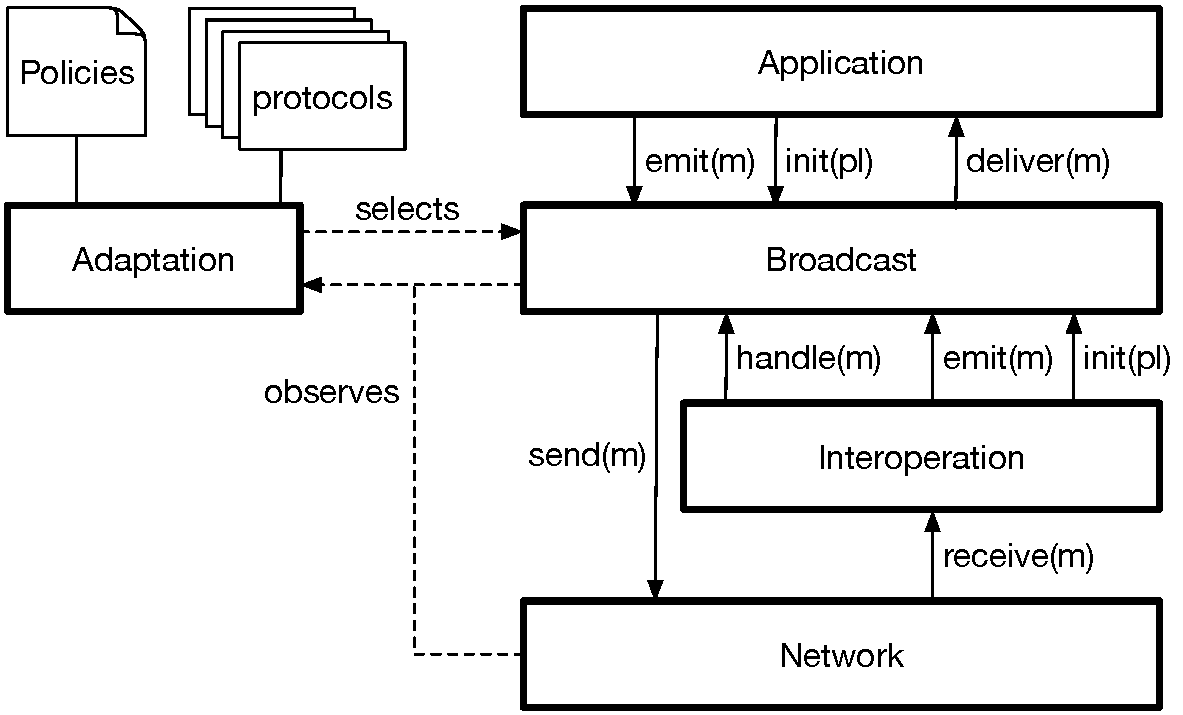
\includegraphics[scale=0.35]{figures/architecture}
	\caption{Architecture of the system}
	\label{fig:system_architecture}
\end{figure}

Second, the Broadcast layer implements a dissemination protocol where a source node sends a message to the entire network by letting nodes act as relays and forward incoming messages.
%
We present in form of API the main operations required by any broadcast protocol:

\begin{itemize}
	\item $\AlgoInit()$: Nodes use this method to create a new message with the payload to disseminate.
	The metadata associated with this payload differs between protocols.
	For instance, a location-based technique may add the emitter's geographic position obtained from a GPS device to the metadata.
	\item $\AlgoEmit()$: Source nodes use this method to initiate a broadcast session.
	\item $\AlgoHandle()$: This method is triggered on every message reception and implements one broadcast protocol. 
\end{itemize}

The third main layer is the MANET application per se and it is placed on the top of the Network and Broadcast layers.
%
When the application requires to disseminate the information $I$, a new broadcast message is created by calling $\AlgoInit()$ with $I$ as argument.
%
The dissemination of $I$ starts with a call to $\AlgoEmit()$, its propagation to others nodes in the network is performed by $\AlgoSend()$ and any message in the interest of the application will be delivered via $\AlgoHandle()$. \er{false, this is with deliver(). handle() is from the network to the bcast protocol}

The architecture of a MANET application is depicted on Figure~\ref{fig:system_architecture} along with two more layers: Interoperation and Adaptation.
%
These two layers extend an application with our adaptive approach in a network of nodes with heterogeneous configurations, by monitoring the dynamics of the network and choosing the best broadcast protocol, accordingly. \er{revise previous sentence, it may seem that the }


\subsection{Framework of adaptation}
\labsection{overview:adaptation_framework}
We are interested in designing an \emph{adaptive} approach to broadcast in MANETs.
%
Adaptation refers to the ability of the system to change its behavior based on the observation of its deployment environment and performance.
%
In our target context, adaptation refers to the ability to dynamically select and configure the protocol used for broadcasting.
%
It is important to note that this adaptation and protocol selection should be possible not only for the entire system but also, just for a part of it.
%
Thus, we must guarantee interoperability among heterogeneous regions of nodes.
%
\er{the following tries to provide more details than is needed here, yet is unclear. This section should provide the high-level of the separation between mechanism and policy and not detail how each work.}
More concretely, every relay node between the source of a broadcast message and each destination node must perform a forward operation, such that there is any lost of messages when the emitter and receiver are not necessarily running the same protocol; our layer of interoperability deals with this regard.

\subsubsection{Interoperation layer}
\labsection{overview:interoperation_layer}

\er{the content of this section is not in the right place. It is not the purpose of the overview section to present the details of how the interoperability and adaptation work. This is done in the two subsequent sections. Overall this section should be half a page, not more.}

We propose an interoperation mechanism between the Network and Broadcast layers, as shown in Figure~\ref{fig:system_architecture}.
%
The basic idea is to broadcast a received message as a source node when the protocol of the emitter and the one form the receiver differ.\vicent{from?}
%
We assume that the protocol identifier is piggybacked on each broadcast message, note that this action does not modify the content of the message nor the metadata use by the protocols to their functioning.
\vicent{"on each broadcast message. Note that this action does not modify the message content, nor the metadata used by ..." }
%
This simple adaptation mechanism is depicted in \refalg{adaptation_mechanism_simple}.
%
The function $\FuncHandler()$ (line~\ref{alg:adaptation_mechanism_simple:receive}) acts as a wrapper for the communication primitive with the same name at the Network Layer.\vicent{Here Layer is in capital but before wasn't. What do you prefer?}
%
When the protocol identifiers of the emitter and receiver nodes differ, a new message will be forward \vicent{forwarded?} keeping the original payload (line~\ref{alg:adaptation_mechanism_simple:init}) but using the receiver's protocol instead (line~\ref{alg:adaptation_mechanism_simple:emit}). This algorithm have a drawback, though a message with the same payload is forwarded twice when the protocol identifiers of two emitters differ.
%
A more efficient adaptation mechanism is shown in \refalg{adaptation_mechanism} where we use timers to delay....
\raziel{TODO:
\begin{itemize}
	\item finish with the description of \refalg{adaptation_mechanism}
	\item argue that these simple and yet efficient mechanism guarantees coverage for any protocol and mention the proof in section 4
	\item create Broadcast super class to reduce the space used by all implementation of broadcast
	\item give an overall overview of the Adaptation layer saying that its detail explanation requires another section
\end{itemize}
}
\er{none of these things belong in section 3.}
